\documentclass{article}
\author{SBHS Science Olympiad, Gold}
\usepackage[margin=.05in, landscape]{geometry}
\setlength{\columnsep}{.1in}
\usepackage{amsmath, multicol}
\usepackage{xcolor}
\usepackage{graphicx, wrapfig, float}

% Symbols
\newcommand{\ddd}{$\bullet$}
% Colors
\newcommand{\red}[1]{\textcolor{red}{#1}}
\newcommand{\green}[1]{\textcolor{green}{#1}}
\newcommand{\blue}[1]{\textcolor{blue}{#1}}
\newcommand{\pink}[1]{\textcolor{magenta}{#1}}
\newcommand{\orange}[1]{\textcolor{orange}{#1}}
\newcommand{\yellow}[1]{\textcolor{yellow}{#1}}
% Headings
% Note: The order of importance is the ROYGBV
\newcommand{\mysection}[1]{\colorbox{yellow}{\textbf{\textit{\red{#1}}}}}
\newcommand{\mysub}[1]{\underline{\textbf{{\textit{\orange{#1}}}}}}
\newcommand{\mysubsub}[1]{{{\green{#1}}}}
\newcommand{\mysubsubsub}[1]{{{\blue{#1}}}}
\newcommand{\vocab}[1]{{\pink{#1}}}
% Pictures
\newcommand{\fig}[1]{
	\includegraphics[width=\columnwidth]{#1}
}
\newcommand{\figwidth}[2]{
	%file, width
	\includegraphics[width=#2cm]{#1}
}
\newcommand{\figwrap}[1]{
	%file, width, height, side
	\begin{wrapfigure}{r}{0.5\textwidth}
		\begin{center}
			\includegraphics[width=0.48\textwidth]{#1}
		\end{center}
	\end{wrapfigure}
}

\begin{document}
	% Uncomment the line below to modify the font size
	 %\small
	 \tiny
	\begin{multicols*}{4}
	
	%Basic Geology	
		\mysection{Glacial Basics}
		\mysub{Aerosol:} a colloidal suspension of particles dispersed in air or gas.
		\mysub{Firn:} the intermediate state between snow and glacial ice
		\mysub{Accumulation:} Accumulation is when glaciers gain more mass through snowfall, windblown snow, avalanches, etc
		\mysub{Ablation:} Ablation is when glaciers loose mass through surface melt, surface meltwater runoff, sublimation, avalanching and windblown snow.
    %Global Connections  
         \mysection{Global Connections}
		\mysub{Atmosphere}
		Past 200 yrs: Past 200 yr: CO2 went up by 40\% and Methane by 200\% - 300\%; Glaciers Reflect heat from the sun; increased dust and soot from grazing, farming, and burning of fossil fuels and forests, are also causing glacier retreat by
		 \ddd Past 200 yr: CO2 went up by 40\% and Methane by 200\% - 300\%, which glaciers have the ability to combat
       \ddd Reflect heat from the sun, 
        \ddd increased dust and soot from grazing, farming, and burning of fossil fuels and forests, are also causing glacier retreat (albedo)
        \ddd layers of dust and soot are darkening the color of glaciers and snowpacks, causing them to absorb more solar heat and melt more quickly, and earlier in spring.
        \ddd \blue{Albedo}, or "whiteness," is a scientific term meaning reflectivity
        \ddd Cooking stoves (biomass stoves) darken snow and ice in mountainous regions. In The himalayas this is bad because the Yangtze, Yellow, Mekong, and Ganges rivers all feed from glaciers
        \ddd 90\% of Himalayan Glacier Melting Caused by Aerosols and Black Carbon
        \ddd \vocab{Aerosol}: a colloidal suspension of particles dispersed in air or gas.
		\textbf{reducing albedo}.
		\begin{wrapfigure}{R}{0.2\textwidth}
			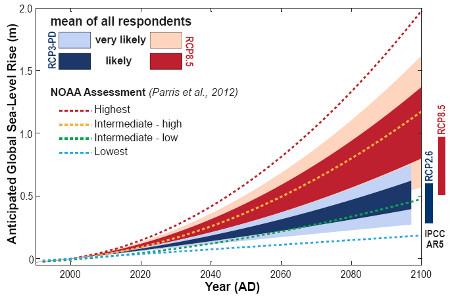
\includegraphics[width=0.1\textwidth]{NOAASeaLevel}
		\end{wrapfigure}
		\mysub{Ocean} If glacier melted 
		\mysubsub{sea level would rise by: } All of Greenland (7.2m); West Antarctic Ice Sheet (3.2m). All of Antarctica (57m). 
         \ddd seal level has risen by 4 to 8 inches over the past century
         \ddd rate of rise over the past 20 years has been 0.13 inches (3.2 millimeters) a year
		\mysub{Lithosphere} When glaciers erode the rock underneath them, they release carbon gases trapped in the lithosphere. Also, when ice sheets weigh down on the sea floor, the cause depression in the earth's lithosphere, and the edges are called fore bulges, which are massive hills that areas like America's east coast lie upon. When these sink, the depressions left rise, causing a reshuffling of the earth's lithosphere. This is called glacial isostatic adjustment.
		\vocab{basal sliding}. when the ice slides over the land with a layer of water acting as a lubricant and reducing the friction between land and ice. pressure from the weight of the ice reduces the melting point at the base of the glacier which allows the ice to melt, allowing water to be present.  glaciers can move in even the coldest of climates.
    %Ice Cores
        \mysection{Ice Cores} a core sample drilled from the accumulation of snow and ice over many years that have recrystallized and have trapped air bubbles from previous time periods, the composition of which can be used to reconstruct past climates and climate change; typically removed from an ice sheet
        \mysub{Oxygen Isotopes}
            \ddd 2 common isotopes $O^16$ and $O^18$
            \ddd Water w/ 16O is lighter, water with 18O is heavier; 16 tends to evaporate easier, causing 18 accumulate in oceans and 16 to end up in water and ice
            \ddd During constant climatic conditions the 16O lost to evaporation returns to the oceans by rain and streams, so that the ratio of 18O to 16O (18O / 16O) is constant.
            \ddd But, during a glaciation, some of the 16O gets tied up in glacial ice and does not return to the oceans. Thus during glaciations the 18O / 16O ratio of sea water increases.
            \ddd During an interglaciation, on the other hand, the 16O that was tied up in glacial ice returns to the oceans causing a decrease in the 18O / 16O ratio of seawater.
            \ddd Thus, we expect that during glaciations the 18O / 16O ratio in seawater will be high, and during interglaciations the 18O /16O ratio in seawater will be low.
        \mysub{Info from Ice Cores}
            \ddd \textbf{Accumulation rate} - The thickness of the annual layers in ice cores can be used to derive a precipitation rate (after correcting for thinning by glacier flow). Past precipitation rates are an important palaeoenvironmental indicator, often correlated to climate change, and it’s an essential parameter for many past climate studies or numerical glacier simulations.
            \ddd \textbf{Melt Layers} - Ice cores provide us with lots of information beyond bubbles of gas in the ice. For example, melt layers are related to summer temperatures. More melt layers indicate warmer summer air temperatures. Melt layers are formed when the surface snow melts, releasing water to percolate down through the snow pack. They form bubble-free ice layers, visible in the ice core
            \ddd \textbf{Past air temperatures} - It is possible to discern past air temperatures from ice cores. This can be related directly to concentrations of carbon dioxide, methane and other greenhouse gasses preserved in the ice.
        \mysection{Sedimentary Sequences}
        \ddd Sedimentary environments are areas where sediments are deposited; glaciers are an example of this
        \mysub{Supraglacial (ice marginal)}
            \ddd Readily be observed along glacial margins
            \ddd A dark, dirty-ice zone is not uncommon at a glacier’s leading edge
            \ddd The supraglacial environment is a very unstable place because material deposited on top of ice is going to move when the ice melts
            \ddd Till-like mixtures of material with a wide range of particle sizes, called \vocab{"diamicton"}
            \ddd Reflect a complex history of deposition
        \mysub{Subglacial}
            \ddd Most difficult to observe. Rely on ice cores and down-hole cameras 
            \ddd glaciers grind up and mix rock and soil debris in and beneath their base forming a mixture of material (rocks, sand, silt, and clay) that is called till
            \ddd \vocab{Till} is the most common subglacial deposit, but river and lake deposits also occur 
        \mysub{Proglacial}
            \ddd even more dynamic than the subaglacial one
            \ddd glacial meltwater and summer rains carry debris away from the glacier or deposit it in lakes that come and go as the force of the water causes natural dams to give way and lakes to drain, sometimes catastrophically sweeping material away in the wate
            \ddd Include materials sorted by water or wind, river sediment (called outwash), lake sediment, windblown sand, and windblown silt called loess
        \mysection{Milankovitch Cycles}
         describe the collective effects of changes in the Earth's movements on its climate over thousands of years. variations in \textit{eccentricity}, \textit{axial tilt}, and \textit{precession} of the Earth's orbit resulted in cyclical variation in the solar radiation reaching the Earth, and that this \textit{orbital forcing} strongly influenced climatic patterns on Earth.
         \mysub{Eccentricity:} refers to the earths orbit and its shift from being circular to more elliptical over time;
        \mysub{Axial Tilt (Obliquity): }Tilt of earths axis of rotation. A greater tilt means more drastic seasons; The angle varies between $22.1^\circ$ and $24.5^\circ$, over a cycle of about 41,000 years. The current tilt is $23.44^\circ$. We are currently on a downward trend, meaning warmer climates.
        \mysub{Axial Precession: } is a gravity-induced, slow, and continuous change in the orientation of an astronomical body's rotational axis. The cycle is relative to fixed starts, with a period of $25771.5$ yrs
        \mysub{Aspidal Precession: }changing of the line between the sun and the earth that changes. Tilt of the orbit itself. 
        \mysubsub{Solar Forcing: }changes in these movements of the Earth, which alter the amount and location of solar radiation reaching the Earth.
        \vocab{Perihelion: }closest to the sun; \vocab{Aphelion: }farthest from the sun; The semi-major axis is a constant, therefore when the earth orbit becomes more eccentric, the semi-minor axis shortens. Increase in \vocab{solar irradiation: }at closest approach to the Sun (perihelion) compared to the irradiation at the furthest distance (aphelion) is slightly larger than four times the eccentricity.
        \vocab{Milutin Milankovic} Serbian geophysicsicts and astronomer.
        \ddd \mysub{how long: }100,000 year long cycle. 
    %History of Ice on Earth
    \mysection{History of Ice on Earth}
    	\mysub{Recent History}
    	There have been five or six major ice ages in the past 3 billion years
    	
    	The Late Cenozoic Ice Age began 34 million years ago, its latest phase being the Quaternary glaciation, in progress since 2.58 million years ago. 
    	
    
        \mysub{Neoproterozoic Snowball on Earth} 
            \vocab{Snowball earth} around \textbf{650 mya}--biological activity in the ocean surface collapsed for millions of years; \textbf{Ended} when volcanic outgassing raised CO2 to 350x modern level; Ocean was virtually covered by thin sea ice + continents were covered in patchy ice due to hydrologic cycle; \vocab{Sir Douglas Mawson} proposed this. 
        \mysub{Late Palezoic Ice Ages}
            \ddd Conventional view: paleozoic ice age was a long ice age for 10 million years w/ some internal waning + waving of glaciers
            \ddd Recent research: series of shorter glacial events separated by periods of warmth
            \ddd Expanded from South America to southern Africa to Australia 
            \ddd The ending constitutes turnover to greenhouse state
            \ddd Sea level response (glacio eustatic) to ice age may be less extreme than once thought
        \mysub{Eocene Oligocene Transition} and the impact of opening oceanic seaways
            \ddd Marked by large scale extinction
            \ddd Most affected organisms were marine or aquatic in nature
            \ddd Major cooling on land and in ocean
            \ddd Causes include volcanic activity + meteorite impacts + decrease in atmospheric CO2
            \ddd Sea level changes mark transition-- in NE Italy, sea level fell 20 m and then 50-60 m in the Oligocene Isotope Event
            \ddd Extinctions could have been caused by volcanic explosions or meteorites
            \ddd Extinction caused by climate change and major fall in sea levels
        \mysub{Pleistocene onset of Northern Hemisphere glaciation}
            \ddd lead to reorganization and relocation of species associations and may have enhanced species turnover
            \ddd Changes in CO2 could have helped to lead to glaciation
            \ddd Began a unique period in Earth’s history where both poles have remained ice locked
            \ddd Between 10 and 6 Ma but did not gain momentum until 3.5-3 Ma
            \ddd Northern Hemisphere glaciation occurred in episodes after Greenland froze
            \ddd Tectonic changes might have triggered more extensive NH glaciation
        \fig{ice_ages1}
		\mysection{Glacial Formation} % New SEction
		\mysub {Glacial Ice:}
		Glacier formation - snow in same area year long and accumulates into masses of ice; ; after the first winter this is known as neve; after two winters, snow turns into firn; the ice increases in density over years
		\mysub{Ice Crystal Structure:} 
		Commonly takes the shape of sheets or planes of oxygen atoms joined in a series of open hexagonal rings; ice can form 18 different crystalline phases; tacked in a laminar structure that occasionally deforms by gliding; When this gliding deformation occurs, the bonds between the layers break, and the hydrogen atoms involved in those bonds must become attached to different oxygen atoms
		\mysub{Properties of Ice:} The albedo is 0.5 to 0.9 for snow, 0.3 to 0.65 for firn, and 0.15 to 0.35 for glacier ice
		\mysubsub{Albedo:} lowers the melting point of the glacier due to hydrostatic pressure, where deeper parts of the glacier are colder
	%Figure intermission
	    \fig{landforms}
        \fig{mtnglacier}
        \fig{moraines}
        \fig{Glacier_Types}
        \fig{hydrology}
        \fig{laurentideicesheet}
        \fig{larsencollapses}
        \fig{glacierflow2}
	%Mass Balance and Flow
		\mysection{Mass-balance and Flow}
		\mysub{Ablation and Accumulation Zones:}
		\mysubsub{Accumulation Zones} are the part of the glacier that has more accumulation than ablation
		\mysubsub{Ablation Zones} are the part of the glacier that has more ablation than accumulation, and the calculate mass balance, just add the two figures
		\fig{AblationAccumulationZones}
		\mysub{Equilibrium Lines} The point across a glacier where accumulation is equal to ablation; The lower the altitude of this line, the faster the glacier advances, and vice versa
		\mysub{Relation of flow to elevation and gradient:}
		\mysubsub{Gradient -} the higher the gradient, the faster the floor of the glacier; Glaciers steeper in maritime climates and temperate latitudes then in continental climates and polar latitudes.
		\mysubsub{Elevation -}Lower the altitude, the less likely it is to find a glacier; So, the lower altitude causes glaciers to be valley or piedmont glaciers rather then cirque, and more active.
    %Glacier Types and Forms
		\mysection{Glacier Types and Forms}
		\mysub{Ice Caps} have an area less than 50,000 square km
		\mysub{Ice Sheets} have an area greater than this; only extant ice sheets are in Antarctica and Greenland
		\mysub{Alpine Glaciers} Begin high in the mountains from cirques and then valley, then piedmont
		\mysubsub{Cirque Glaciers} glacial ice collected in bowl shaped depression high in the mountains 
		\mysubsub{Hanging Glaciers}  A hanging glacier originates high on the wall of a glacial valley and descends only part of the way to the surface of the main glacier and abruptly stops, typically at a cliff.
		\mysubsub{Piedmont Glaciers} valley glaciers that spread out onto a flat lowland
		\mysubsub{Tidewater Glaciers} glaciers that flow to the sea
		\mysubsub{Valley Glaciers} a thin stream of ice that takes up a valley and originates from one or many cirques
		\mysubsub{Apron Glaciers} Glaciers that cling to steep mountainsides and are very avalanche prone.
	%Glacial Features
	    \mysection{Glacial Features}  
	    \mysub{Ice Stream} section of fast flow within a glacier that make up most o the way that a glacier discharges ice and sediment.
		\mysub{Ice Shelves} a suspended section of ice connected to a landmass that forms when a glacier flows down to the ocean’s surface.
		\mysub{Ice Rise} an obvious dome shaped bump in the ice of a glacier formed when the seabed under a glacier has a similar bump, located with valley glaciers.
		\mysub{Ice Stream} a long, narrow sheet of ice that extends out over the ocean that forms when a valley glacier moves very rapidly onto the ocean.
		\mysub{Nunatak} an exposed, often rocky element of a ridge, mountain, or peak not covered with ice or snow within an ice field or glacier; also called glacial islands.
		\mysub{Crevasses} deep cracks in glacier ice caused by the stress of the ice moving over rocky terrain underneath, indicate that glacier is under different types of stress as it flows. If crevasses close up, it shows that a glacier is flowing over an area of less gradient. 
		\mysub{Ogives} alternating bands of light and dark ice that forms ridges arcs of ice bending downstream. This shows that a glacier is moving faster in the center, creating these arched bands, or is moving over steeper terrain.
		\mysub{Ice Falls} glaciers flow over an steep drop or squeeze through an narrow place characterized by rapid flow and a crevassed surface. Happens when a glacier flows over a steep surface or narrows.
	%Hydrology
	    \mysection{Hydrology}
	        \ddd Glacier hydrology is the study of the flow of water through glaciers
            \ddd Glacier ice is permeable, with a network of microscopic veins and lenses of water.
            \mysub{Glacier Permeability} 
                \ddd The rate at which water percolates through the glacier is dependent on salinity, pressure and temperature. 
                \ddd  The rate at which ice seeps through the ice, however, is so slow, that for practical reasons ice can generally be considered impermeable
            \mysub{Supraglacial (surface) water} on a glacier is formed by the ice melting during the summer.
            \mysub{Ablation}: Surface melt; occurs in hard packed snow (firn: the transistional state between snow and ice)
            \mysub{Swamp zone} If a firn becomes saturated all the way to the surface it becomes a ‘swamp zone’; Swamp zone moved up glacier as the melt season progresses.
            \ddd Much of the meltwater runoff in Antarctica is restricted to coastal areas and ice shelves during the summer seasons
            \mysub{Englacial Hydrology}
                \ddd \vocab{Moulins} are vertical shafts cut by the water.
                \ddd Water cascades down these into the ice sheet. Despite the pressures within the ice sheet, moulins remain open by constant melting by the water
            \mysub{Subglacial Hydrology}
                \ddd Basal meltwater flowing through large subglacial networks impact glacial erosion and ice velocity. 
            \mysub{Proglacial Drainage}
                \ddd Abundant meltwater can form large braided river plains, or sandur
                \ddd Runoff is less in Antarctica, and meltwater in the northern Antarctic Peninsula tends to be restricted to small braided streams
                \ddd These streams redeposit glacial sediments and rework glacial landforms
        \mysection{Laurentide Ice Sheet}
            \ddd The mass of ice in the Greenland Ice Sheet has begun to decline. From 1979 to 2006, summer melt on the ice sheet increased by 30 percent, reaching a new record in 2007
            \ddd Antartica has not shown noticeable changes. 
            \ddd Antartic peninsula has seen changes which is the part that sticks out of the continent
        \mysection{Methods of studying glaciers}
        \fig{mbMeas}
            \ddd The two main processes used to determine ablation or accumulation are \textbf{probing} and \textbf{crevasse stratigraphy}, which can give accurate measurements of snowpack thickness.
            \mysub{Probing}: researchers will place poles in the icepack at various points, at the beginning of the melt period or accumulation period. After a few months the researchers will return and look at the changes in levels of ice, by looking at the height of the ice along the pole.
            \mysub{Crevasse stratigraphy}: researchers will find crevasses, then observe the number of layers that formed. Based on the layers the researchers will be able to determine how much snow accumulated. The layers are almost like layers in a tree trunk.
            \mysub{Cosmogenic nuclide dating} is useful for directly dating rocks on the Earth’s surface. It gives an Exposure Age: that is, how long the rock has been exposed to cosmic radiation. It is effective on timescales of several millions of years. It assumes that boulders have not been buried and then re-exposed at the Earth’s surface.
            \mysub{Radiocarbon dating} dates the decay of Carbon-14 within organic matter. Organic matter needs to have been buried and preserved for this technique. It is effective for up to the last 40,000 years. It assumes that organic material is not contaminated with older radiocarbon (which, for example, is a common problem with organic material from marine sediment cores around Antarctica).
            \mysub{Amino Acid Racemisation} dates the decay and change in proteins in organisms such as shells.
            \mysub{Optically Stimulated Luminescence} dates the radiation accumulated in quartz or feldspar grains within sand. The radiation emanates from radioactive grains within the sediment, such as zircons. It is effective for hundreds of thousands of years, and dates how long the sediment has been buried.
        \mysection{Recent Records of Cryospheric Change}
            \vocab{Cryosphere}: portions of Earth’s surface where water is in solid form including sea ice, lake ice, river ice, snow cover, glaciers, ice caps, ice sheets, and frozen ground (which includes permafrost).
            \mysub{Larsen Ice Shelf}
                a long ice shelf in the northwest part of the Weddell Sea, extending along the east coast of the Antarctic Peninsula from Cape Longing to Smith Peninsula
                \ddd The collapse of Larsen B has revealed a thriving chemotrophic ecosystem 800 m (half a mile) below the sea.
                \ddd 31 January 2002 - March 2002 Larsen B sector partially collapsed and parts broke up. 
                \ddd Larsen B was stable for 10,000 years, but due to warm currents eating away the underside of the shelf it collapsed. 
                \ddd 3,250-square-kilometer (1,255-square-mile) section collapsed (size of Rhode island)
                \fig{Larsen_contours} \\
            \mysub{Kilimanjaro}
                \ddd Kilimanjaro's shrinking northern glaciers, thought to be 10,000 years old, could disappear by 2030
                \ddd The northern ice field, which holds most of the remaining glacial ice, lost more than 140 million cubic feet of ice in the past 13 years
                \ddd Approximately 29\% of the volume and 32\% of the surface area of the ice sheet has been lost since 2000.
                \ddd No real reason is known, with possible links to global warming and less snowfall
            \mysub{Amundsen Sea Embayment}
                \ddd is located off of west Antarctica and the ice that drains into it is roughly 3 km thick
                \ddd Recently, this sheet has significantly thinned because of shifts in wind patterns that allow warmer water to flow under the ice, and is already melting enough to raise the global sea level by 0.2 mm per year. 
                \ddd Two of Antarctica's largest glaciers drain into this basin and if they were to melt, the sea level could increase by up to 3 yards. 
                \ddd The weak underbelly of the West Antarctic Ice Sheet, and if it were to collapse, could destabilize the entire west antarctic ice sheet
 	    \mysection{Post-Glacial Landscape}  
	 	    \mysub{Erosional Features:}
	 	    \mysubsub{Cirques} a bowl shaped basin formed when a glacier erodes under the bergschrund(a crevasse at or near the head of a glacier) which opens in the early summer, exposing the rock underneath to frost action and causes upper rock to avalanche and scour the floor beneath in the bowl shape, or the bowl left behind from a cirque glacier.
	 	    \mysubsub{Tor} a free-standing rock outcropping that abruptly rises from the surrounding environment, formed at first by erosion and weathering of the ground surrounding it.
	 	    \mysubsub{U-Shaped Valley} happen when valley glaciers advance, eroded a u-shaped depression in the land, and then recede, leaving this U-shaped valleys and mountains behind.
	 	    \mysubsub{Hanging Valley} as a smaller glacier at a higher elevation joins a lower, but larger valley glacier, and they recede, the u shaped valley created by the smaller glaciers opens up onto the lower depression formed by the larger glacier.
	 	    \mysubsub{Aretes} a sharp, crested ridge that separates the heads of two opposing cirques where glaciers used to reside and carved this thin ridge.
	 	    \mysubsub{Horns}when glaciers erode three or more aretes, ending with sharp, vertical peak.
	 	    \mysubsub{Stritations/Grooves} are carved into bedrock as glaciers pass over it.
	 	    \mysubsub{Rôche moutonnée} occurs when a glacier claws itself up a hill, it damages the surface, leaving jagged and irregular on that side, but as it slides down, it polishes the surface, leaving the other side of the same rock smooth and even.
	 	    \mysubsub{Tarn} a lake left in a bowl shaped depression by a receding cirque glacier.
	 	    \mysub{Depositional Features: }
			\mysubsub{Moraines} are rocks or sediment deposited by a glacier, typically at its edges.
			\mysubsubsub{End/Terminal} a moraine that forms at the leading edge of a glacier marking its furthest advance, formed by debris pushed to the front of a glacier.
			\mysubsubsub{Recessional} a series of ridges formed parallel to the terminal moraine and form when a glacier temporarily stops receding.
			\mysubsubsub{Lateral} a series of parallel ridges deposited along the sides of a glacier that form when frost shatters the valley walls and causes them to collapse.
			\mysubsubsub{Medial}  a ridge of a moraine that forms in the center of a valley. It forms when two glaciers meet and the debris on the edges of the adjacent valley sides join and are carried on top of the enlarged glacier.
			\mysubsubsub{Ground} an irregular blanket of sediment most often deposited by continental glaciers
			\mysubsub{Kettles} when a block of ice calves and is submerged into sediment, and subsequently melts, the hole it leaves behind is called a kettle.
			\mysubsub{Kames} a hill of sand, sediment and till that forms on top of a retreating glacier then is deposited on the land underneath as the glacier further melts.
			\mysubsub{Drumlins} an elongated hill shaped like a inverted spoon aligned with the ice flow that forms under the glacier bed and a left when the glacier retreats.
			\mysubsub{Eskers} a long ridge composed of sediment and gravel formed under a glacier when subglacial rivers in ice walled tunnels left sediment underneath then and when the retaining walls of ice melted away
			\mysubsub{Erratics} pieces of rocks that are foreign to their surroundings regarding their size and type. They are transported by glaciers for thousands of miles.
			\mysubsub{Moulins} are vertical shafts created in a glacier by waater within it.
        \mysection{Category?}
            \mysub{Ice ages}
                \ddd An ice age is a long interval of time (millions to tens of millions of years) when global temperatures are relatively cold and large areas of the Earth are covered by continental ice sheets and alpine glaciers. Within an ice age are multiple shorter-term periods of warmer temperatures when glaciers retreat (called interglacials or interglacial cycles) and colder temperatures when glaciers advance (called glacials or glacial cycles).
                \ddd At least five major ice ages have occurred throughout Earth’s history: the earliest was over 2 billion years ago, and the most recent one began approximately 3 million years ago and continues today (yes, we live in an ice age!).
                \ddd Currently, we are in a warm interglacial that began about 11,000 years ago. The last period of glaciation, which is often informally called the “Ice Age,” peaked about 20,000 years ago. At that time, the world was on average probably about $ 10^\circ F (5^\circ C) $ colder than today, and locally as much as $ 40^\circ F (22^\circ C) $ colder.
            \mysub{What causes ice ages?}
                \ddd Many factors contribute to climate variations, including changes in ocean and atmosphere circulation patterns, varying concentrations of atmospheric carbon dioxide, and even volcanic eruptions. The following discusses key factors in (1) initiating ice ages and (2) the timing of glacial-interglacial cycles.
                \ddd One significant trigger in initiating ice ages is the changing positions of Earth’s ever-moving continents, which affect ocean and atmospheric circulation patterns. When plate-tectonic movement causes continents to be arranged such that warm water flow from the equator to the poles is blocked or reduced, ice sheets may arise and set another ice age in motion.
                \ddd Today’s ice age most likely began when the land bridge between North and South America (Isthmus of Panama) formed and ended the exchange of tropical water between the Atlantic and Pacific Oceans, significantly altering ocean currents.
            \mysub{How does ice build up?}
                \ddd Throughout the Quaternary period, high latitude winters have been cold enough to allow snow to accumulate. It is when the summers are cold, (i.e., summers that occur when the sun is at its farthest point in Earth's orbit), that the snows of previous winters do not melt completely. When this process continues for centuries, ice sheets begin to form. Finally, the shape of Earth's orbit also changes. At one extreme, the orbit is more circular, so that each season receives about the same amount of insolation. At the other extreme, the orbital ellipse is stretched longer, exaggerating the differences between seasons. The eccentricity of Earth's orbit also proceeds through a long cycle, which takes 100,000 years. Major glacial events in the Quaternary have coincided when the phases of axial tilt, precession of equinoxes and eccentricity of orbit are all lined up to give the northern hemisphere the least amount of summer insolation.
            \mysub{Glacial History of Quaternary}
                The Quaternary System is that lasted from the present to approximately 2.588 million years ago with the Neogene system before the Quaternary. The Quaternary System contains two series: the Holocene and the Pleistocene with the Holocene being the present. In this period, ice sheets were able to form in Greenland and Antarctica and the continents were formed to their present shape. As glaciers formed and later retreated, thousands of lakes and rivers were created all over the world. As the glaciers retreated the sea level rose and the amount of biological diversity in the oceans increased
                \fig{Quelccaya_Glacier}
                \fig{series}
     \mysection{Glacier Fluctuations}
	        \ddd In ~1930 Milutin Milankovitch proposed that variations in three parameters of the earth's orbit caused glacial fluctuations: 
	        \ddd 1.	Orbital eccentricity - the orbit of the earth around the sun is not a circle, but is elliptical and also varies. This eccentricity is a minor cause for seasons.
	        \ddd 2.	Tilt variations in the axis of rotation (obliquity) - the tilt of the earth's rotational axis varies with time. A tilted axis is the primary cause of seasons. This varies between 22.1 and 24.5 in a 40,000 year cycle
	        \ddd 3.	Precession - the earth's axis of rotation wobbles which results in minor fluctuations in the amount of solar radiation we receive.
	        \ddd Milankovitch pacing seems to best explain glaciation events with periodicity of 100k, 40k, and 20k years. This pattern seems to fit the info on climate change found in oxygen isotope cores. However, there are some problems with the Milankovitch theories.
	        \ddd \textbf{100,000 year Problem eccentricity} variations have a significantly smaller impact on solar forcing than precession or obliquity and may be expected to produce the weakest effects. The greatest observed response is at the 100k year timescale, while the theoretical forcing is smaller at this scale, in regard to the ice ages. During the last 1 million years, the strongest climate signal is the 100k year cycle.
	        \ddd \textbf{400,000 year Problem} (aka stage 11 problem) eccentricity variations have a strong 400k year cycle. That cycle is only clearly present in climate records older than the last million years.
	        \ddd Stage 5 problem refers to the timing of the penultimate interglacial that appears to have begun 10k years in advance of the solar forcing hypothesized to have caused it.
	        \ddd Effect exceeds cause climate behavior is much more intense than calculated variations. Various internal characteristics of climate systems are believed to be sensitive to the insolation changes, causing amplification(positive feedback) and damping reponses(negative feedback)
	        
        \pagebreak
        \mysection{Where are glaciers found?}
            \ddd Antarctica:	\pink{ }
            \ddd Greenland:	1,784,000
            \ddd Canada: 200,000
            \ddd Central Asia:	109,000
            \ddd Russia:	82,000
            \ddd United States:	75,000 (including Alaska)
            \ddd China and Tibet:	33,000
            \ddd South America: 25,000
            \ddd Iceland:	11,260
            \ddd Scandinavia:	2,909
            \ddd Alps: 2,900
            \ddd New Zealand:	1,159
            \ddd Mexico: 11
            \ddd Indonesia:	7.5
            \ddd Africa: 10
   %Current Glaciers and Facts
		\mysection{Current Glacier Records:} 
		    \mysub{Top Five Longest Non-Polar}
		    \mysubsub {Fedchenko Glacier} in Tajikistan at 77 km
		    \mysubsub {Siachen Glacier}, in the Karakorum range, border between India and Pakistan - 76 km
		    \mysubsub {Biafo Glacier} in Pakistan also by the border - 67 km
		    \mysubsub {Bruggen Glacier} in Chile - 66 km
		    \mysubsub {Baltoro Glacier} in Pakistan at the border - 63 km. \mysub{Longest per continent: } 
		    \mysubsub {Lambert Glacier(Biggest in the world)} in Antarctica(320 mi long, 40 mi wide)
		    \mysubsub {Heard Island Glacier} in Australia(which cover 67 percent of heard island proper)
		    \mysubsub {Siachen Glacier} in Asia with 3 trillion cubic tons of ice
		    \mysubsub {Kilimanjaro's glaciers} in Africa(which are retreating alarmingly)
		    \mysubsub {Vatnojokull Glacier} of Europe (Iceland --> covers 8 percent)
		    \mysubsub {Perito Moreno Glacier} in S.A. which is thriving despite trend of retreat in the globe
		    \mysubsub {Hubbard Glacier} in N.A. (largest tidewater glacier my far). 
		    \mysubsub{Europe Glaciers} found in the Alps, Caucasus and the Scandinavian Mountains and Iceland. Most of Europe's large glaciers are in Norway, with the exception of the biggest, which is in Iceland, called the Vatnojokull Glacier.
		    \mysubsub{N.A. Glaciers} Glaciers are in 9 of America's states, in Mexico and of course in Canada. Southernmost in the states is the Lilliput in California. Glaciers in Mexico are in the Pico de Orizaba (Citlaltépetl), Popocatépetl and Iztaccíhuatl, the three tallest mountains in the country.
		    \mysubsub{S.A. Glaciers} S.A. glacier exclusively on the Andes. Apart from this there is a wide range of latitudes on which glaciers develop from 5000 m in the Altiplano mountains and volcanoes to reaching sea level as San Rafael Lagoon ($ 45^\circ $ S) and southwards. South America hosts two large ice fields, the Northern and Southern Patagonian Ice Fields.
		    \mysubsub{Oceania Glaciers} No glaciers remain on the Australia mainland or Tasmania.Heard Island glaciers are located in the territory of Heard Island and McDonald Islands. New Guinea has the Puncak Jaya glacier. New Zealand contains many glaciers,  located near the Main Divide of the Southern Alps in the South Island. They are classed as mid-latitude mountain glaciers. There are eighteen small glaciers in the North Island on Mount Ruapehu.
		    \mysubsub{Africa Glaciers} Only all-season glaciers exsist on Kilimanjaro, Mount Kenya, and the Rwenzori, but seasonally occur in the Drakensberg Range of South Africa, the Stormberg Mountains, and the Atlas Mountains in Morocco.
		    \mysubsub{Antartican Glaciers} Has many outlet glaciers, valley glaciers, cirque glaciers, tidewater glaciers and ice streams e.g. Pine Island Glacier. 
		    \mysub{Quick Facts: }
		    \mysubsub{Fresh Water} has 69 percent of the world's supply in glaciers
		    \mysubsub{Number} of glaciers in Alaska is over 100,000
		    \mysubsub{Glacier} and ice sheet all melted = a sea level rise of over 300 feet
		    \mysubsub{Speed} of glaciers is as high as moving 150 feet per day
		    \mysubsub{A single} glacier ice crystal can grow to the size of a baseball
	\mysection{Vocabulary} 
		\ddd
        Ablation Area: The area of a glacier where more glacier mass is lost than gained\ddd
        Ablation Hollows: Depressions in the snow surface caused by the sun or warm, gusty wind\ddd
        Ablation Moraine: Mound or layer of moraine in the ablation zone of a glacier; the rock has been plucked from the mountainside by the moving glacier and is melting out on the ice surface\ddd
        Ablation Season: Period during which glaciers lose more mass than they gain; usually coincides with summer\ddd
        Ablation Zone: Area or zone of a glacier where snow and ice ablation exceed accumulation\ddd
        Accumulation Area: Area of a glacier where more mass is gained than lost\ddd
        Accumulation Season: Period during which a glacier gains more mass than it loses usually coincides with winter\ddd
        Accumulation Zone: Area of a glacier where more mass is gained than lost\ddd
        Advance: When a mountain glacier’s terminus extends farther down valley than before; glacial advance occurs when a glacier flows down valley faster than the rate of ablation at its terminus\ddd
        Alpine Glacier: A glacier that is confined by surrounding mountain terrain; also called a mountain glacier \ddd
        Arête: Sharp, narrow ridge formed as a result of glacial erosion from both sides \ddd 
        Band Ogives: Alternate bands of light and dark on a glacier; usually found below steep narrow icefalls and thought to be the result of different flow and ablation rates between summer and winter\ddd
        Basal Sliding: The sliding of a glacier over bedrock\ddd
        Bergschrund: (Rimaye) Crevasse that separates flowing ice from stagnant ice at the head of a glacier\ddd
        Branched-Valley Glacier: Glacier that has one or more tributary glaciers that flow into it; distinguished from a simple valley glacier that has only a single tributary glacier\ddd
        Catchment Glacier: A semi permanent mass of firn formed by drifted snow behind obstructions or in the ground; also called a snowdrift glacier or a drift glacier\ddd
        Chattermarks: Striations or marks left on the surface of exposed bedrock caused by the advance and retreat of glacier ice\ddd
        Cirque: Bowl shaped or amphitheater usually sculpted out of the mountain terrain by a cirque glacier\ddd
        Cirque Glacier: Glacier that resides in basins or amphitheaters near ridge crests; most cirque glaciers have a characteristic circular shape, with their width as wide or wider than their length\ddd
        Cold Glacier: Glacier in which most of the ice is below the pressure melting point; nonetheless the glacier’s surface may be susceptible to melt due to incoming solar radiation, and the ice at the rock/ice interface may be warmed as a result of the natural (geothermal) heat from the earth’s surface\ddd
        Compression Flow: Flow that occurs when glacier motion is decelerating down-slope\ddd
        Constructive Metamorphism: Snow metamorphism that adds molecules to sharpen the corners and edges of an ice crystal\ddd
        Crevasse: Open fissure in the glacier surface\ddd
        Crevasse Hoar: A kind of hoarfrost; ice crystals that develop by sublimation in glacial crevasses and in other cavities with cooled space and calm, still conditions under which water vapor can accumulate; physical origin is similar to depth hoar\ddd
        Dead Ice: Any part of a glacier which has ceased to flow; dead ice is usually covered with moraine\ddd
        Dirt Cone: A cone-shaped formation of ice that is covered by dirt; a dirt cone is caused by a differential pattern of ablation between the dirt-covered surface and bare ice\ddd
        Drain Channel: Preferred path for meltwater to flow from the surface through a snow cover\ddd
        Drift Glacier: A semi-permanent mass of firn formed by drifted snow behind obstructions or in the ground; also called a catchment glacier or a snowdrift glacier\ddd
        Drumlin: Remnant elongated hills formed by historical glacial action; it is not clear exactly how they are formed and why they form only in some glaciated regions\ddd
        Dump Moraine: A mound or layer of moraine formed along the edge of a glacier by rocks that fall off the ice; sometimes called a ground moraine\ddd
        End Moraine: An arch-shaped ridge of moraine found near the end of a glacier\ddd
        Equilibrium Zone: Zone of a glacier in which the amount of precipitation that falls is equal to the amount that melts the following summer\ddd
        Esker: A sinuous ridge of sedimentary material (typically gravel or sand) deposited by streams that cut channels under or through the glacier ice\ddd
        Extending flow: when glacier motion is accelerating down-slope\ddd
        False ogives: bands of light and dark on a glacier that were formed by rock avalanching\ddd
        Fjord: glacial troughs that fill with seawater\ddd
        Foliation: layering in glacier ice that has distinctive crystal sizes and/or bubbles; foliation is usually caused by stress and deformation that a glacier experiences as it flows over complex terrain, but can also originate as a sedimentary feature\ddd
        Forbes bands: alternate bands of light and dark on a glacier; usually found below steep narrow icefalls and thought to be the result of different flow and ablation rates between summer and winter\ddd
        Forel stripes: shallow, parallel grooves on the face of a large melting ice crystal\ddd 
        Geyser: Fountain that develops when water from a conduit is forced up to the surface of a glacier; also called a negative mill\ddd
        Glacial advance: when a mountain glacier's terminus extends farther downvalley than before; occurs when a glacier flows downvalley faster than the rate of ablation at its terminus\ddd
        Glacial Erratic: a boulder swept from its place of origin by glacier advance or retreat and deposited elsewhere as the glacier melted; after glacial melt, the boulder might be stranded in a field or forest where no other rocks of its type or size exist\ddd
        Glacial grooves: grooves or gouges cut into the bedrock by gravel and rocks carried by glacial ice and meltwater; also called glacial striations\ddd
        Glacial retreat: when the position of a mountain glacier's terminus is farther upvalley than before; occurs when a glacier ablates more material at its terminus than it transports into that region\ddd
        Glacial striations: grooves or gouges cut into the bedrock by gravel and rocks carried by glacial ice and meltwater; also called glacial grooves\ddd
        Glacial till: accumulations of unsorted, unstratified mixtures of clay, silt, sand, gravel, and boulders; the usual composition of a moraine\ddd
        Glacial trough: a large u-shaped valley formed from a v-shaped valley by glacial erosion\ddd
        Glaciated: land covered in the past by any form of glacier is said to be glaciated\ddd
        Glacier: a mass of ice that originates on land, usually having an area larger than one-tenth of a square kilometer; many believe that a glacier must show some type of movement; others believe that a glacier can show evidence of past or present movement\ddd
        Glacier cave: a cave of ice, usually underneath a glacier and formed by meltwater; cave entrances are often enlarged near a glacier terminus by warm winds; most common on stagnant portions of glaciers\ddd
        Glacier fire: a phenomenon in which strong reflection of the sun on an icy surface causes a glacier to look like it is on fire\ddd
        Glacier flood: a sudden outburst of water released by a glacier\ddd
        Glacier flour: a fine powder of silt- and clay-sized particles that a glacier creates as its rock-laden ice scrapes over bedrock; usually flushed out in meltwater streams and causes water to look powdery gray; lakes and oceans that fill with glacier flour may develop a banded appearance; also called rock flour\ddd
        Glacier ice: well-bonded ice crystals compacted from snow with a bulk density greater than 860 kilograms per cubic meter (55 pounds per cubic-foot)\ddd
        Glacier mill: a nearly vertical channel in ice that is formed by flowing water; usually found after a relatively flat section of glacier in a region of transverse crevasses\ddd
        Glacier pothole: potholes formed at the bottom of glaciers through erosion caused by sand and gravel in melt-water; melt-water seeps through crevasses in the glaciers, sometimes forming whirlpools; at the bottom of the glacier, the water is under very high pressure, leading to erosion of underlying rocks\ddd
        Glacier remainie: a glacier that is reconstructed or reconstituted out of other glacier material; usually formed by seracs falling from a hanging glacier, then re-adhering; also called reconstituted, reconstructed or regenerated glacier\ddd
        Glacier snout: the lowest end of a glacier; also called glacier terminus or toe\ddd
        Glacier sole: the bottom of the ice of a glacier\ddd
        Glacier table: a rock that resides on a pedestal of ice; formed by differential ablation between the rock-covered ice and surrounding bare ice\ddd
        Glacier terminus: the lowest end of a glacier; also called glacier snout or toe\ddd
        Glacier toe: the lowest end of a glacier; also called glacier snout or terminus\ddd
        Glacier trough: u-shaped valleys transformed from v-shaped stream valleys due to erosion caused by passing glaciers\ddd
        Glacieret: a very small glacier\ddd
        Glacierized: land overlaid at present by a glacier is said to be covered; the alternative term glacierized has not found general favour\ddd
        Ground moraine: continuous layer of till near the edge or underneath a steadily retreating glacier\ddd
        Hanging glacier: a glacier that terminates at or near the top of a cliff\ddd
        Hanging valley: a valley formed by a small glacier that has a valley bottom relatively higher than nearby valleys formed by larger glaciers\ddd
        Headwall: a steep cliff, usually the uppermost part of a cirque\ddd
        Horn: a peak or pinnacle thinned and eroded by three or more glacial cirques\ddd
        Ice apron: a mass of ice adhering to a mountainside\ddd
        Ice cap: a dome-shaped mass of glacier ice that spreads out in all directions; an ice cap is usually larger than an icefield but less than 50,000 square kilometers (12 million acres)\ddd
        Ice cave: a cave of ice, usually underneath a glacier and formed by meltwater; cave entrances are often enlarged near a glacier terminus by warm winds; most common on stagnant portions of glaciers\ddd
        Ice covered: land overlaid at present by a glacier is said to be covered; the alternative term glacierized has not found general favor\ddd
        Ice divide: the boundary separating opposing flow directions of ice on a glacier or ice sheet\ddd
        Ice Dome: ice surface with parabolic surface; located in accumulation zone \ddd 
        Ice quake: a shaking of ice caused by crevasse formation or jerky motion\ddd
        Ice sheet: a dome-shaped mass of glacier ice that covers surrounding terrain and is greater than 50,000 square kilometers (12 million acres), the Greenland and Antarctic ice sheets)\ddd
        Ice stream: (1) a current of ice in an ice sheet or ice cap that flows faster than the surrounding ice (2) sometimes refers to the confluent sections of a branched-valley glacier (3) obsolete synonym of valley glaciers\ddd
        Ice-cemented glacier: a rock glacier that has interstitial ice a meter or so below the surface\ddd
        Ice-cored glacier: a rock glacier that has a buried core of ice\ddd
        Icefall: part of a glacier with rapid flow and a chaotic crevassed surface; occurs where the glacier bed steepens or narrows\ddd
        Ice field: a mass of glacier ice; similar to an ice cap, and usually smaller and lacking a dome-like shape; somewhat controlled by terrain\ddd
        Jokulhlaup: (1) a large outburst flood that usually occurs when a glacially dammed lake drains catastrophically (2) any catastrophic release of water from a glacier\ddd
        Lateral moraine: a ridge-shaped moraine deposited at the side of a glacier and composed of material eroded from the valley walls by the moving glacier\ddd
        Marginal crevasse: a crevasse near the side of a glacier formed as the glacier moves past stationary valley walls; usually oriented about 45 degrees up-glacier from the side wall\ddd
        Medial moraine: a ridge-shaped moraine in the middle of a glacier originating from a rock outcrop, nunatak, or the converging lateral moraines of two or more ice streams\ddd
        Meltwater conduit: a channel within, underneath, on top of, or near the side of a glacier that drains meltwater out of the glacier; usually kept open by the frictional heating of flowing water that melts the ice walls of the conduit\ddd
        Moraine: a mound, ridge, or other distinct accumulation of glacial till\ddd
        Moraine shoal: glacial moraine that has formed a shallow place in water\ddd
        Moulin: a nearly vertical channel in ice that is formed by flowing water; usually found after a relatively flat section of glacier in a region of transverse crevasses; also called a pothole\ddd
        Mountain glacier: a glacier that is confined by surrounding mountain terrain; also called an alpine glacier\ddd
        Negative mill: a geyser; a fountain that develops when water from a conduit is forced up to the surface of a glacier\ddd
        Niche glacier: very small glacier that occupies gullies and hollows on north-facing slopes (northern hemisphere); may develop into cirque glacier if conditions are favorable\ddd
        Nunatak: a rocky crag or small mountain projecting from and surrounded by a glacier or ice sheet\ddd
        Ogives: alternate bands of light and dark ice seen on a glacier surface\ddd
        Outburst flood: any catastrophic flooding from a glacier; may originate from trapped water in cavities inside a glacier or at the margins of glaciers or from lakes that are dammed by flowing glaciers\ddd
        Outlet glacier: a valley glacier which drains an inland ice sheet or ice cap and flows through a gap in peripheral mountains\ddd
        Patterned grounds: consists of mostly symmetrical geometries displayed across the ground surface in relation to local frost action and cryogenic processes. Patterns emerge as a result of surface disturbances caused by thermal anomalies and freeze processes such as frost heave. Frost heave will disturb the frost layer as ice lenses accumulate and protrude, causing unstable soil conditions. Can be polygons, circles, stripes, nets, and steps. \ddd
        Paternoster lakes: a series of tarns connected by a single stream or a braided stream system\ddd
        Periglacial: relating to or denoting an area adjacent to a glacier or ice sheet or otherwise subject to repeated freezing and thawing \ddd        
        Piedmont glacier: large ice lobe spread out over surrounding terrain, associated with the terminus of a large mountain valley glacier\ddd
        Pingo: also called hydrolaccolith or bulgunniakh, is a mound of earth-covered ice found in the Arctic and subarctic that can reach up to 70 metres in height and up to 600 m in diameter. \ddd       
        Polar glacier: a glacier entirely below freezing, except possibly for a thin layer of melt near the surface during summer or near the bed; polar glaciers are found only in polar regions of the globe or at high altitudes\ddd
        Pothole: a nearly vertical channel in ice that is formed by flowing water; usually found after a relatively flat section of glacier in a region of transverse crevasses; also called a moulin\ddd
        Push moraine: moraine built out ahead of an advancing glacier\ddd
        Randkluft: a fissure that separates a moving glacier from its headwall rock; like a bergschrund\ddd
        Reconstituted glacier: a glacier that is reconstructed or reconstituted out of other glacier material; usually formed by seracs falling from a hanging glacier then re-adhering; also called reconstructed glacier, regenerated glacier, or glacier remainie\ddd
        Reconstructed glacier: a glacier that is reconstructed or reconstituted out of other glacier material; usually formed by seracs falling from a hanging glacier then re-adhering; also called reconstituted glacier, regenerated glacier, or glacier remainie\ddd
        Regelation: motion of an object through ice by melting and freezing that is caused by pressure differences; this process allows a glacier to slide past small obstacles on its bed\ddd
        Regenerated glacier: a glacier that is reconstructed or reconstituted out of other glacier material; usually formed by seracs falling from a hanging glacier then re-adhering; also called reconstituted or reconstructed glacier, or glacier remainie\ddd
        Retreat: when a mountain glacier's terminus doesn't extend as far downvalley as it previously did; occurs when ablation surpasses accumulation\ddd
        Retreating glacier: a glacier whose terminus is increasingly retreating upvalley compared to its previous position due to a higher level of ablation compared to accumulation\ddd
        Rock flour: a fine powder of silt- and clay-sized particles that a glacier creates as its rock-laden ice scrapes over bedrock; usually flushed out in meltwater streams, causing water to look powdery gray; lakes and oceans that fill with glacier flour may develop a banded appearance\ddd
        Rock glacier: looks like a mountain glacier and has active flow; usually includes a poorly sorted mess of rocks and fine material; may include: (1) interstitial ice a meter or so below the surface (“ice-cemented”), (2) a buried core of ice (“ice-cored”), and/or (3) rock debris from avalanching snow and rock\ddd
        Rogen Moraine: A Rogen moraine (also called ribbed moraine) is a subglacially (i.e. under a glacier or ice sheet) formed type of moraine landform, that mainly occurs in Fennoscandia, Scotland, Ireland and Canada. They cover large areas that have been covered by ice, and occur mostly in what is believed to have been the central areas of the ice sheets \ddd
        Sastrugi: parallel wave-like ridges caused by winds on the surface of hard snow, especially in polar regions. \ddd
        Sedimentary ogives: alternating bands of light and dark at the firn limit of a glacier; the light bands are usually young and lightest at the highest level up-glacier, becoming increasingly older and darker as they progress down-glacier\ddd
        Serac: an isolated block of ice that is formed where the glacier surface is fractured\ddd
        Sichelwannen- curved grooves formed by water under immense pressure at the base of a glacier \ddd
        Sintering: the bonding together of ice crystals\ddd
        Snowdrift glacier: a semipermanent mass of firn formed by drifted snow behind obstructions or in the ground; also called a catchment glacier or a drift glacier\ddd
        Splay crevasse: a crevasse pattern that forms where ice slowly spreads out sideways; commonly found near a glacier terminus\ddd
        Sub polar glacier: a glacier whose temperature regime is between polar and temperate; usually predominantly below freezing, but could experience extensive summer melt\ddd
        Surging glacier: a glacier that experiences a dramatic increase in flow rate, 10 to 100 times faster than its normal rate; usually surge events last less than one year and occur periodically, between 15 and 100 years\ddd
        Tarn: a small mountain lake or pool; a mountain lake formed in a cirque excavated by a glacier. A moraine may form a natural dam below a tarn\ddd
        Terminus: the lowest end of a glacier, also called the glacier toe or glacier snout\ddd
        Thomson crystal: a large ice crystal found in deep, stagnant water-filled cavities of a glacier\ddd
        Tidewater glacier: mountain glacier that terminates in the ocean\ddd
        Tongue: a projection of the ice edge up to several km in length caused by wind and current; usually forms when a valley glacier moves very quickly into a lake or ocean\ddd
        Tributary glacier: a small glacier that flows into a larger glacier\ddd
        Valley glacier: a mountain glacier whose flow is confined by valley walls\ddd
        Wave ogives: ogives that show some vertical relief on a glacier; usually the dark bands are in the hollows and the light bands are in the ridges; form at the base of steep, narrow ice falls\ddd
        Weathered ice: glacier ice that has been exposed to sun or warm wind so that the boundaries between ice crystals are partly disintegrated\ddd
	   	
	\end{multicols*}
\end{document}